\documentclass{tufte-handout}

%\geometry{showframe}% for debugging purposes -- displays the margins

\usepackage{amsmath}

% Set up the images/graphics package
\usepackage{graphicx}
\setkeys{Gin}{width=\linewidth,totalheight=\textheight,keepaspectratio}
\graphicspath{{graphics/}}

\title{Analysis of RPGLite data}
\author[]{Tom Wallis \& William Kavanagh}
\date{April 2020}  % if the \date{} command is left out, the current date will be used

\usepackage{hyperref}
\hypersetup{
    colorlinks=true,
    linkcolor=blue,
    filecolor=magenta,      
    urlcolor=cyan,
}

% The following package makes prettier tables.  We're all about the bling!
\usepackage{booktabs}

% The units package provides nice, non-stacked fractions and better spacing
% for units.
\usepackage{units}

% The fancyvrb package lets us customize the formatting of verbatim
% environments.  We use a slightly smaller font.
\usepackage{fancyvrb}
\fvset{fontsize=\normalsize}

% Small sections of multiple columns
\usepackage{multicol}

% Provides paragraphs of dummy text
\usepackage{lipsum}

\usepackage[obeyFinal,textsize=footnotesize]{todonotes}

% These commands are used to pretty-print LaTeX commands
\newcommand{\doccmd}[1]{\texttt{\textbackslash#1}}% command name -- adds backslash automatically
\newcommand{\docopt}[1]{\ensuremath{\langle}\textrm{\textit{#1}}\ensuremath{\rangle}}% optional command argument
\newcommand{\docarg}[1]{\textrm{\textit{#1}}}% (required) command argument
\newenvironment{docspec}{\begin{quote}\noindent}{\end{quote}}% command specification environment
\newcommand{\docenv}[1]{\textsf{#1}}% environment name
\newcommand{\docpkg}[1]{\texttt{#1}}% package name
\newcommand{\doccls}[1]{\texttt{#1}}% document class name
\newcommand{\docclsopt}[1]{\texttt{#1}}% document class option name

\newcommand{\WilliamToDo}[1]{\todo[color=cyan]{\textbf{W:~{#1}}}}
\newcommand{\TomToDo}[1]{\todo[color=orange]{\emph{T:~{#1}}}}

\begin{document}

\maketitle% this prints the handout title, author, and date

\begin{abstract}
\noindent This document describes the data generated by the RPGLite experiment, the analysis we have performed on it thus far and areas where we should like to perform further analysis
\end{abstract}

%\printclassoptions

\section{The Data}


Data\footnote{this may not be a necessary section to include, though it may be useful if this document is to be used as a reference for \textit{outsiders}.} is collected in the form of a Mongo database and organised into six collections of similar documents detailed here with their notable fields:
\begin{enumerate}
    \item \textbf{games}: in progress games
    \begin{itemize}
        \item usernames -- an array of the usernames for players 1 and 2 respectively,
        \item start\_time -- python datetime object given moment of game creation to millisecond precision,
        \item Moves -- list of moves made in notation of the form $pxC^1pyC^2\_nn$ which would denote player $x \in \{1,2\}$ using character $C^1 \in \{K,A,R,H,W,B,M,G\}$  to attack player $y$'s character $C^2$ and rolling $nn \in \{0..99\}$ 
    \end{itemize}
    \item \textbf{completed\_games}: games now completed
        \begin{itemize}
        \item as above.
        \item winner -- {1,2} denoting winner if one was found (can be non present if game was abandon)
    \end{itemize}
    \item \textbf{page\_hits}:
    \item \textbf{player\_backup}
    \item \textbf{players}:
    \item \textbf{special\_data}:
\end{enumerate}

\section{Initial Analysis}

\subsection{win-delta / pick-rate}\footnote{The three figures described here are all generated by running \textit{rolling\_analysis.py}}

A common form for game analytics, also known as pick-rate/win-rate, win-delta / pick-rate (herein WD/PR) plots game material in a way that allows for easy comparison of how popular and powerful they are. WD/PR is commonly used as the basis for balance changes, however it is flawed. Whilst it does give a good account of material which should be tweaked to bring it more in line with the rest, it does not account for personal preference or represent mismatches between specific material. 

\begin{figure}
    \centering
    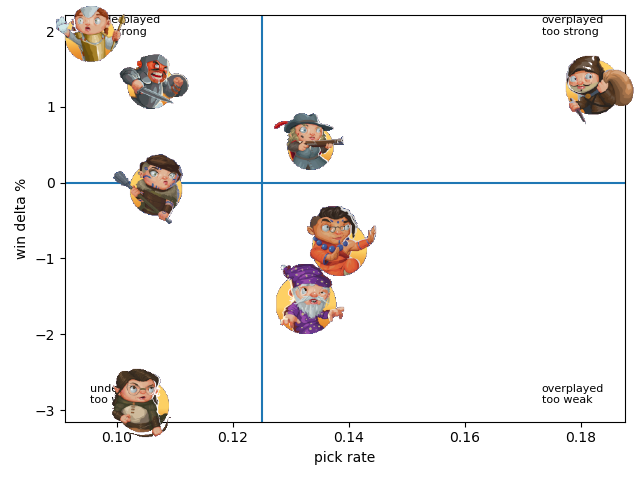
\includegraphics{pick-win.png}
    \caption{WD/PR generated 14-4, 10 days after initial release. Guidelines are drawn at x=0.125 or 1/8 as that is what would be the value if each were chosen equally, and at y = 0\% as that would be the value of material that wins as often as it loses.}
    \label{fig:WD/PR}
\end{figure}

% Lad, I can't get this warning to buzz off.

Fig. ~\ref{fig:WD/PR}~shows that the Healer is both the most successful material and the least popular. \href{'https://staticctf.akamaized.net/J3yJr34U2pZ2Ieem48Dwy9uqj5PNUQTn/2MXEODt9QteOU3WGh4vmNE/51261bebfc558521b7411ccb78ece4fb/Y5S1_Matrix_Attackers.png'}{There are examples of this peculiar occurrence in other games.} Perhaps the low popularity makes the win-delta value more volatile, or the players are choosing based on factors other than their effectiveness. However popularity should be balanced for just as effectiveness is, as game designer Jeff Kaplan states, \textit{"The perception of balance is more powerful than balance itself."}

As our previous work pertains to metagame development, we wanted to investigate if we could use WD/PR variants to measure this development over time. To do this we have plotted WD/PR for every day since release. 

\begin{figure}
    \centering
    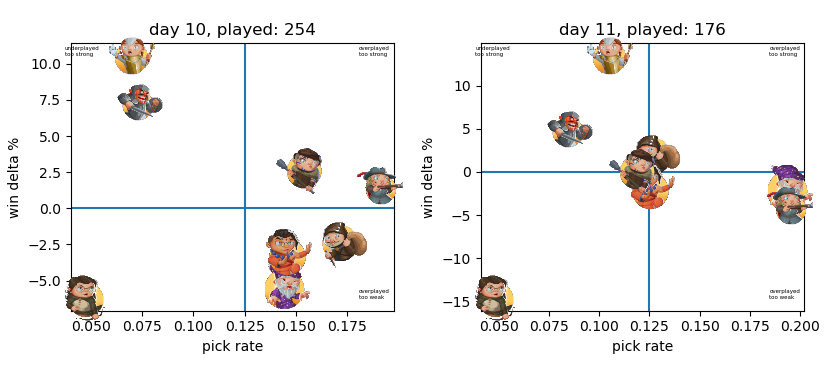
\includegraphics{pick-win-per-day-snipped.PNG}
    \caption{Snippet of WD/PR over days}
    \label{fig:my_label}
\end{figure}

As a measure of how \textit{settled} the metagame is, we plotted each character on their own axes with their WD/PR values over days. Between each point there is a vector giving the disparity between points, the average of these vectors between each day should give a good indication of how \textit{settled} the metagame is.

\begin{figure}
    \centering
    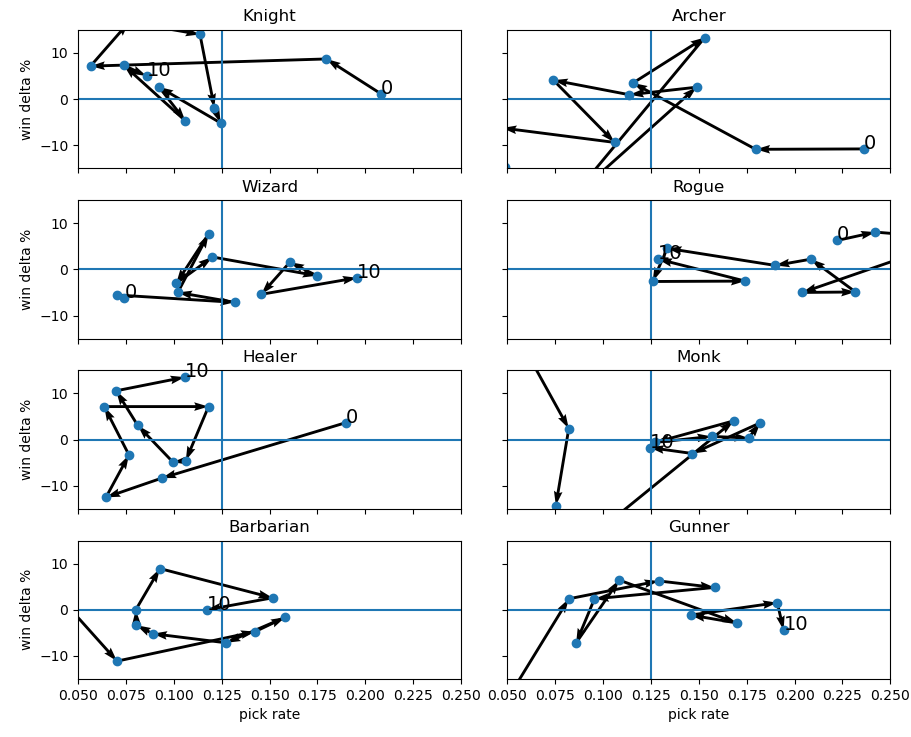
\includegraphics{pick-win-per-char.png}
    \caption{WD/PR, per character, over days}
    \label{fig:my_label}
\end{figure}

\subsection{Elo and non-skill factors on placement}

RPGLite has two systems for player ranking, \textit{skill}, a measure of our own creation which is public to all players, and \textit{Elo}, which we also measure, but that we do not make public. Elo is a standard mechanism for measuring player skill, devised for Chess in the 1950s. It forms the basis for a lot of competitive matchmaking ranking systems used today, including \textit{TrueSkill} developed by Microsoft \footnote{For more on Elo, TrueSkill and competitive matchmaking, \href{https://www.microsoft.com/en-us/research/wp-content/uploads/2006/10/Game-Developer-Feature-Article-Graepel-Herbrich.pdf}{this Microsoft white paper} is a good source.}. Elo is a far better measure of player skill than the "friendly" measure of \textit{skill} which rewards games played over success. 

\begin{figure}
    \centering
    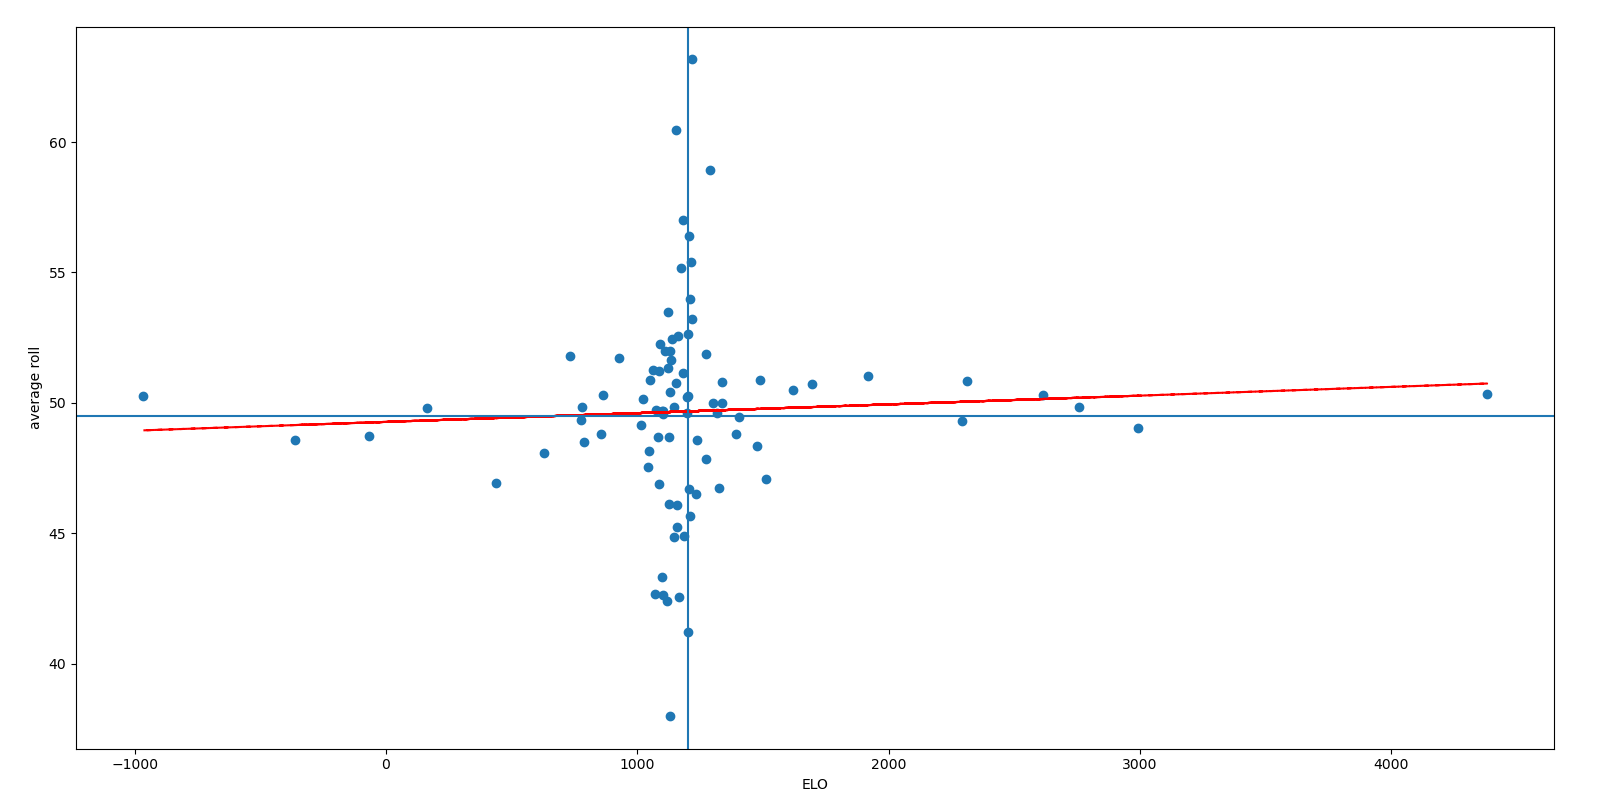
\includegraphics{luck_over_Elo.png}
    \caption{Elo of the playerbase plotted against luck}
    \label{fig:luck-over-Elo}
\end{figure}

We can show that there is a relationship between Elo and the average roll in the player-base, this stands to reason.

It should also be mentioned that RPGLite does have an issue with first-move bias, due to its simplistic nature. A testament to this is that from the first 1653 games completed, 982 were won by the player going first, or 59.4\%.

\subsection{Skill}

This work is devised specifically so that we can say of any given move made in the game whether or not it was \textit{correct}, and if it was not, then what the \textit{cost} of playing the move was. The values referred to here are the optimal values (or \textit{minimax} values), the probability of winning given your opponent tries to minimise the probability of you winning and you try to maximise it. Through exhaustive state exploration we can attribute to every possible action, in every reachable state, for every configuration of the game, a single value of their optimal probability of winning. When faced with a decision to make, the players optimal probability of winning is equivalent to that of when they have chosen to take the optimal action from that state, before the outcome is determined (i.e. before the action has succeeded or failed). Should they take a different action where their optimal probability of winning is less having chosen an action than it was before, then they have chosen a \textit{sub-optimal} action and the difference between their current and past optimal values can be considered the \textit{cost} of the move. A rudimentary measure of how skilful a player is at RPGLite is to average the cost of every move made in every game they have played. In Fig. \ref{fig:cost-over-Elo} we show that there is a relationship between this rudimentary measure of skill and a player's Elo value, which unsurprisingly implies that skill is a factor in success.

\begin{figure}
    \centering
    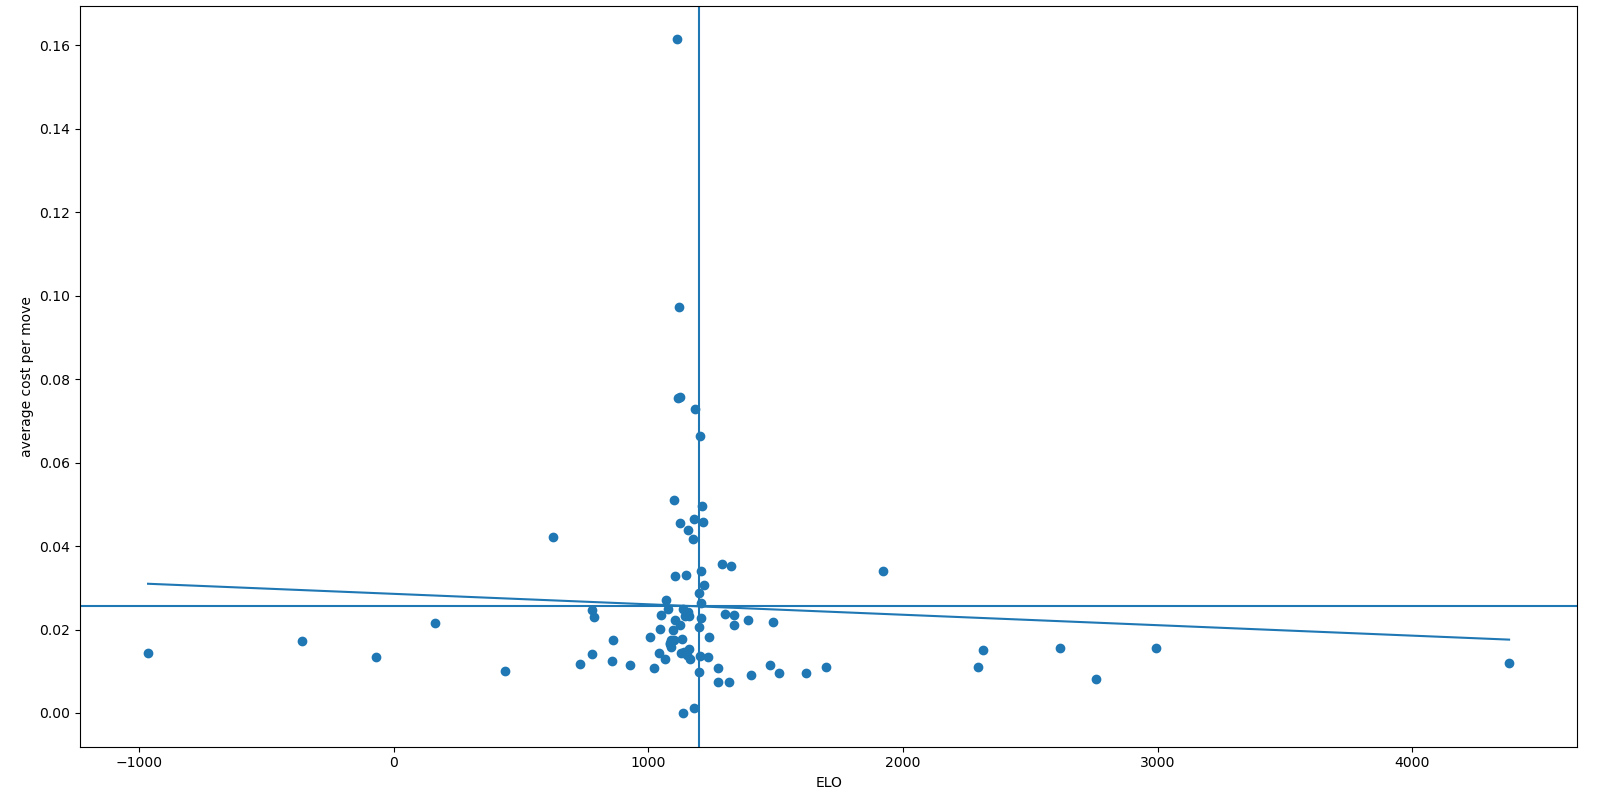
\includegraphics{cost_over_Elo.png}
    \caption{Elo of the playerbase plotted against skill}
    \label{fig:cost-over-Elo}
\end{figure}

\subsection{Player types}

By considering the experience of the player when looking at character selection we can investigate what characters players \textit{learn} to play. Fig. \ref{fig:char-select-by-exp}~can be recreated by user$\_$picks$\_$over$\_$time.py

\begin{figure}
    \centering
    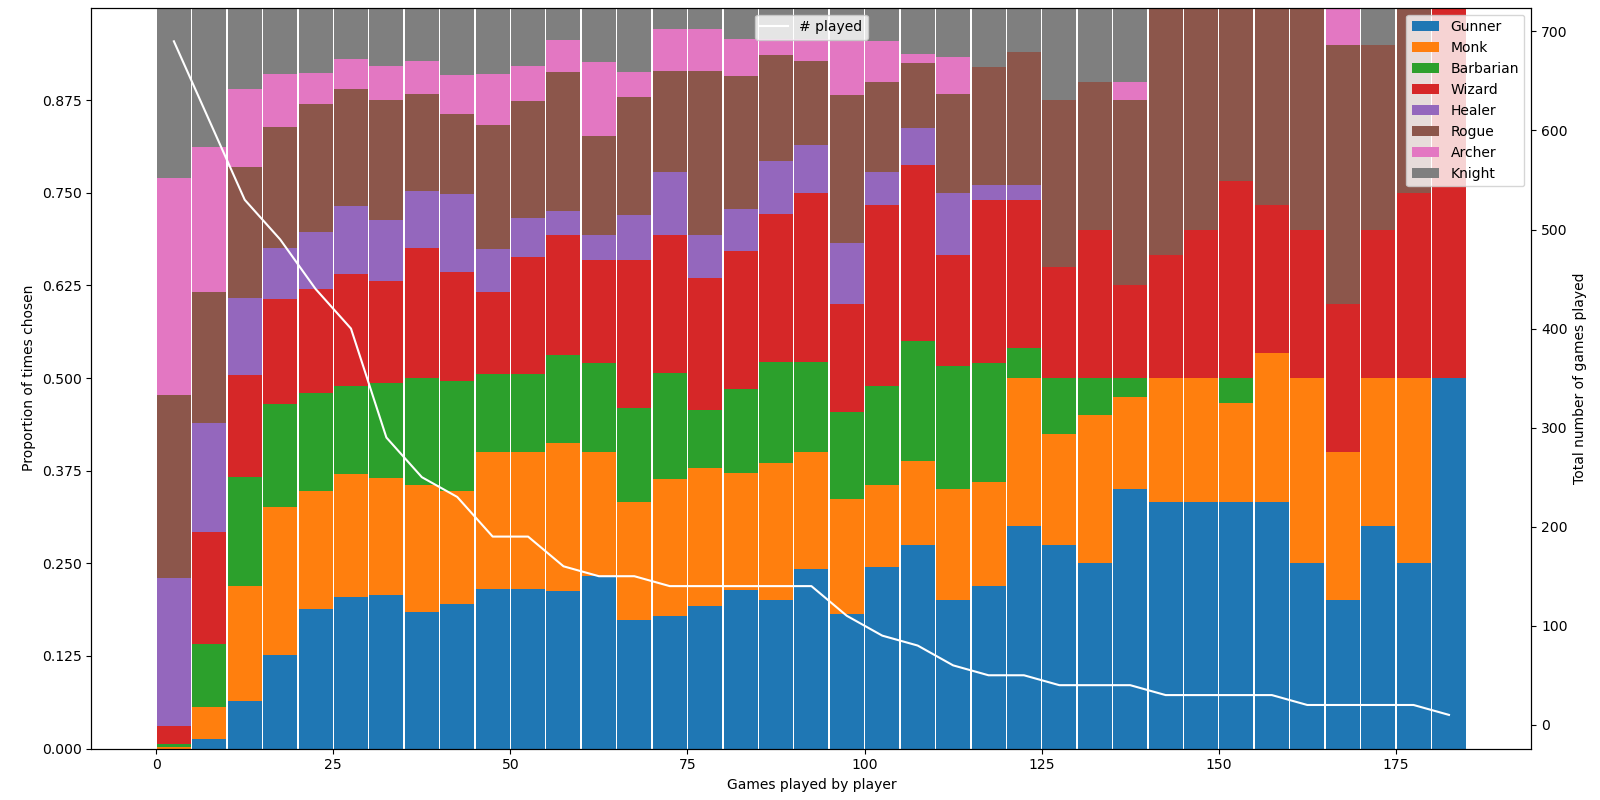
\includegraphics{character_selection_by_games_played.png}
    \caption{Proportion of characters chosen by players of various experience, in 5 game intervals. The number of games played in each interval is also shown to show values that may be less accurate.}
    \label{fig:char-select-by-exp}
\end{figure}

\subsection{Predictive value of chained strategy generation}

Are we good? How good are we? Let's find out.

\end{document}

